\documentclass[a4paper,11pt]{article}
\usepackage[english]{babel}
\usepackage{float}
\usepackage{amssymb}
\usepackage{alltt}
\usepackage{verbatim}
\usepackage{fancyheadings}
\usepackage[latin1]{inputenc}
\usepackage{epsfig}
\usepackage{wrapfig}
\usepackage{lscape}
\usepackage{multicol}
\usepackage{longtable}
\usepackage{vmargin}
\usepackage{graphics}
\usepackage[hang,small,bf]{caption}

\def\TestLength{\\
  \framebox[\voffset]{$\strut$\hfill}\ voffset\\
  \framebox[\hoffset]{$\strut$\hfill}\ hoffset\\
  \framebox[\evensidemargin]{$\strut$\hfill}\ evensidemargin\\
  \framebox[\oddsidemargin]{$\strut$\hfill}\ oddsidemargin\\
  \framebox[\topmargin]{$\strut$\hfill}\ topmargin\\
  \framebox[\headheight]{$\strut$\hfill}\ headheight\\
  \framebox[\headsep]{$\strut$\hfill}\ headheight\\
  \framebox[\topskip]{$\strut$\hfill}\ topskip\\
  \framebox[\footskip]{$\strut$\hfill}\ footskip\\
  \framebox[\footheight]{$\strut$\hfill}\ footheight\\
}

% -----------------------------------------------
% H O R I S O N T A L   A D J U S T M E N T
% -----------------------------------------------
\setlength{\hoffset}{-2.7cm}  % Calibration for personal HP Laserjet4
\setlength{\oddsidemargin}{3.5cm}
\setlength{\textwidth}{14.5cm}

% -----------------------------------------------
% V E R T I C A L   A D J U S T M E N T
% -----------------------------------------------
\setlength{\voffset}{-2.7cm}  % Calibration for personal HP Laserjet4
\setlength{\topmargin}{3cm}
\setlength{\headsep}{.8cm}
\setlength{\footskip}{1.5cm}
\setlength{\textheight}{21.5cm}

\renewcommand{\sectionmark}[1]%
                {\markright{\thesection\ #1}}
\lhead[\fancyplain{}{\bfseries\thepage}]%
      {\fancyplain{}{\bfseries\rightmark}}
\rhead[\fancyplain{}{\bfseries\leftmark}]%
      {\fancyplain{}{\bfseries\thepage}}

\pagestyle{fancyplain}
\renewcommand{\descriptionlabel}[1]%
   {\hspace{\labelsep}\textsf{#1}}

\renewcommand{\contentsname}{Indhold}
\renewcommand{\appendixname}{Appendiks}
\renewcommand{\tablename}{Tabel}
\renewcommand{\figurename}{Figur}

% Inds�t forfatternavn
\author{Tommy Petersen \\
  AIA \\
  Denmark \\
  \texttt{tp@aia.dk} \\
  Copyright 2020 AIA \\
  All rights reserved}

\date{}

% Inds�t dokumentets titel
\title{dax}

\begin{document}

% Generer titel
\maketitle

% -----------------------------------------------
% S E L V E   D O K U M E N T E T
% -----------------------------------------------

% Declarations:

\newcommand{\R}{\mathbb{R}}
\newcommand{\Q}{\mathbb{Q}}
\newcommand{\Z}{\mathbb{Z}}
\newcommand{\N}{\mathbb{N}}

\newtheorem{theorem}{Theorem}[section]
\newtheorem{lemma}{Lemma}[section]
\newtheorem{algorithm}{Algorithm}[section]
\newtheorem{proposition}{Proposition}[section]
\newtheorem{definition}{Definition}[section]
\newtheorem{example}{Example}[section]
\newcommand{\qed}{\nobreak \ifvmode \relax \else
      \ifdim\lastskip<1.5em \hskip-\lastskip
      \hskip1.5em plus0em minus0.5em \fi \nobreak
      \vrule height0.75em width0.5em depth0.25em\fi}

\abstract{
This article presents ideas for an explorative unit.
}

\section{Introduction}
The ability to explore seems crucial to many species.\hfill\break\break
Two features characterize exploration:
\begin{description}
        \item[$\cdot$ Mapping] The environment is mapped in order obtain
                               a model of it.
        \item[$\cdot$ Action] Actions are take in order to update and/or expand
                              the environment model.
\end{description}
This article presents ideas for an explorative unit. The unit is called {\bf dax}
(data explorer) and is suitable for use in a larger compound of explorative units.

\section{dax data flow diagram}
A diagram representing the data flow around dax is shown in
figure~\ref{fig:daxDiagram}.
\begin{figure}[ht]
  \begin{center}
  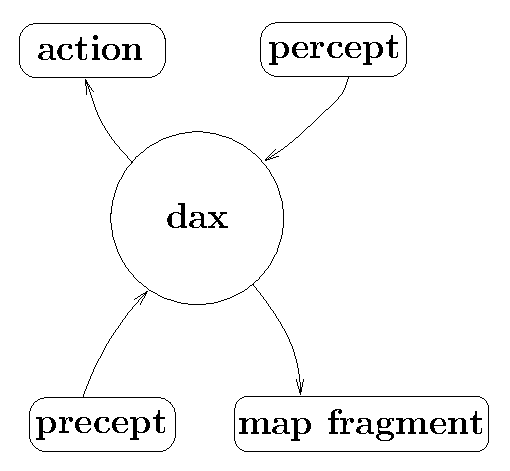
\includegraphics[width=0.33\textwidth, keepaspectratio]
                  {Eps/daxDiagram.eps}
  \end{center}
  \caption{dax data flow diagram.}
  \label{fig:daxDiagram}
\end{figure}
\hfill\break
The data named ``{\bf map fragment}'', ``{\bf action}'', ``{\bf percept}''
and ``{\bf precept}'' are all finite symbol sequences and should be understood
as follows:
\begin{description}
        \item[$\cdot$ map fragment] Part of a map of the environment.
        \item[$\cdot$ action] Chosen action.
        \item[$\cdot$ percept] Sensory data from the environment.
        \item[$\cdot$ precept] Programmed data.
\end{description}
Programmed via the precept, dax continually maps and acts as a result
of a never ending stream of percepts from the environment.

\section{Context concept}
In order to describe what is happening in the dax data flow diagram
(figure~\ref{fig:daxDiagram}), some concepts are defined.

The {\bf model} is defined as a finite symbol sequence. The
model is dax's internal model of the environment. The model
can be updated by concatenating percepts and/or precepts to it.

The model can be structured using the concepts of context and
instance as defined in the following:
\begin{definition}
(context and instance) \hfill\break
A {\bf context} is a suffix having
at least one matching substring within the model.
Such a matching substring must not be the suffix itself and is
called an {\bf instance}.
\label{def1}
\end{definition}
Example:\hfill\break
$$
model = 11010
$$
$$
percept = 110
$$
$$
updated\ model = 11010110
$$
In the model, the longest context and its only instance are as follows:
\hfill\break
\begin{figure}[ht]
  \begin{center}
  \includegraphics[width=0.2\textwidth, keepaspectratio]
                                        {Eps/contextConcept.eps}
  \end{center}
  \label{fig:contextConcept}
\end{figure}
\hfill\break
Having defined context and instance, the two exploration features
{\bf mapping} and {\bf action} can now be defined as will be done in the
following sections.

\section{Map fragment}
In order to describe how dax maps its environment, the concept of a map
fragment is defined.
\begin{definition}
(map fragment) \hfill\break
A map fragment is a pair of the form
$$
(C, D)
$$
where $C$ and $D$ both are finite symbol sequences. $C$ is interpreted as a
context and $D$ is interpreted as data within that context.
\end{definition}
When a chosen context instance and the context itself are spaced by at least
one symbol, a map fragment can be created.
This is done by letting $C$ be the context and
by letting $D$ be the substring beginning immediately after the chosen instance
and ending immediately before the chosen context.
Consider the example:
$$
model = 00101111
$$
$$
percept = 10
$$
$$
updated\ model = 0010111110
$$
\hfill\break
Using the context $10$ and its instance, the structured updated model is
$$
00\framebox{$10$}1111 | 10
$$
\hfill\break
The map fragment is $(10, 1111)$ with $C$ equal to $10$ and $D$ equal to $1111$.

\section{Model location}
Consider again the example:
$$
model = 00101111
$$
$$
percept = 10
$$
$$
updated\ model = 0010111110
$$
\hfill\break
Using the context $10$ and its instance, the structured updated model is
$$
structured\ updated\ model = 00\framebox{$10$}1111 | 10
$$
The substring from the beginning of the model to the last symbol of the
instance is the current location in the internal model of the environment
given the context. The current location is shown in the following:
$$
current\ location = \underline{0010}1111 | 10
$$
\hfill\break
Having obtained the current location in the environment model, dax
must now ready itself to receive new input from the environment
situated in this location. This is done by discarding what
comes after the location in the model. The updated model is then
$$
updated\ model = 0010
$$
Dax is then ready to receive new input from the environment in the form of
a new percept or a new precept.
\hfill\break

\section{Action}
The context instance and the context itself can be spaced zero or
negatively (they overlap). Dax uses this situation to choose an action.

The following example shows a situation where the instance and the context are
zero spaced:
$$
model = 10
$$
$$
percept = 10
$$
$$
updated\ model = 1010
$$
\hfill\break
The structured updated model is as follows:
\hfill\break
\begin{figure}[ht]
  \begin{center}
  \includegraphics[width=0.12\textwidth, keepaspectratio]
                                        {Eps/zeroSpaced1.eps}
  \end{center}
  \label{fig:zeroSpaced1}
\end{figure}
\hfill\break
As can be seen above, the zero spacing between
the instance and the context implies that the model ends with a pattern
which repeats itself at least two times.

The following example shows a situation where the instance and
the context are negatively spaced (they overlap):
$$
model = 110
$$
$$
percept = 000
$$
$$
updated\ model = 110000
$$
\hfill\break
The context and the instance are as follows:
\hfill\break
\begin{figure}[ht]
  \begin{center}
  \includegraphics[width=0.12\textwidth, keepaspectratio]
                                        {Eps/overlappingInstances1.eps}
  \end{center}
  \label{fig:overlappingInstances1}
\end{figure}
\hfill\break
The instance overlaps the context by the sequence $00$.

\subsection{Chosen action}
This section shows how dax uses zero or negative spacing to choose an
action.

First, a lemma, to help argue about what can be expected when the
instance and the context have negative spacing, in other words, when they
overlap.
\begin{lemma}
(the overlap lemma)\hfill\break
If the instance and the context overlap, then their union will end with
a pattern which repeats itself at least two times.\hfill\break
{\bf Proof}.\hfill\break
See figure~\ref{fig:overlappingInstances3} which applies in general to all
overlapping identical substrings.\hfill \qed
\end{lemma}
\begin{figure}[ht]
  \begin{center}
  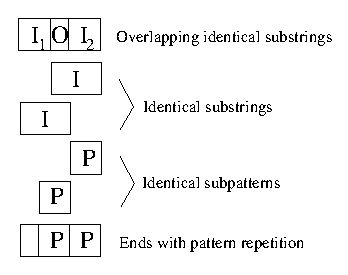
\includegraphics[width=6cm,height=4cm]{Eps/overlappingInstances3.eps}
  \end{center}
  \caption{Proof of the overlap lemma.}
  \label{fig:overlappingInstances3}
\end{figure}

The above shows that dax can expect a future input of periodic
characteristic in case of negative or zero spacing of the instance and
the context. But a periodic input is not desired for an explorative unit
as dax is. It should find new things not repetitions and hence should
rather be in a situation where it can make a map fragment.
So, in an attempt to get to a mapping situation, dax
then chooses an action in the same way as it chooses the data part
when making a map fragment. The action will thus be encoded as the
symbol sequence beginning immediately after the instance and immediately
before the context and will therefore be in the opposite direction than
the data part of the map fragment. Using the previous example with
$$
model = 110
$$
$$
percept = 000
$$
$$
updated\ model = 110000
$$
The structured updated model is
$$
11\framebox{$0|00$}0
$$
so that the chosen action is $0000$. Choosing the action is an attempt
to stop the seemingly periodic behaviour. The model therefore needs
to be updated since the pattern of periodic behaviour is no longer
valid. The substring in the model which precisely contains the action is
a valid representation of the periodic pattern and is therefore removed
from the model. This results in the updated model
$$
updated\ model = 11
$$
After having chosen an action and updated its model, dax awaits a
new percept or a new precept.

\section{No previous substring}
There might be no previous substring of any suffix in the model.
In this case, as per definition~\ref{def1}, the context is undefined
and hence does not exist. The following shows an example:
$$
model = 0
$$
$$
percept = 1
$$
$$
updated\ model = 01
$$
\hfill\break
In this case, dax does not update the model based on context.

\section{Precept}
The {\bf precept} is programmed data. Via the precept, dax can
be programmed both initially and on the fly. The precept expands
the model to the left with the leftmost symbol of the precept
being placed leftmost and the rightmost symbol being placed rightmost in
dax's experience. The following shows an example:
$$
model = 01100
$$
$$
precept = 001
$$
$$
updated\ model = 00101100
$$
The structured updated model:
\hfill\break
$$
00|1011\framebox{$00$}
$$
\hfill\break
The two features of exploration ``{\bf mapping}'' and ``{\bf action}'' also
apply for the precept---by using the opposite directions of those which are used
in the percept described above.

\section{Flow}
Having described the details of the dax data flow diagram in 
figure~\ref{fig:daxDiagram}, the flow can now be summarized as in
figure~\ref{fig:flow}:
\hfill\break
\begin{figure}[ht]
  \begin{center}
  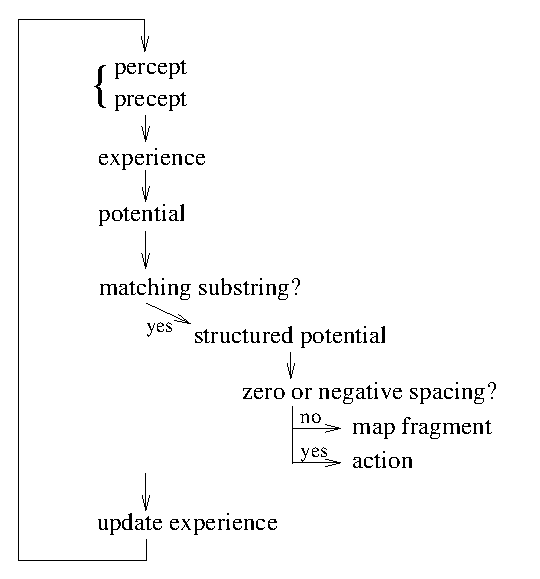
\includegraphics[width=0.43\textwidth, keepaspectratio]
                                        {Eps/flow1.eps}
  \end{center}
  \caption{Flow.}
  \label{fig:flow}
\end{figure}
\hfill\break


\end{document}
